\chapter{Introduction}
Particle accelerators occupy a key role both in fundamental research and in all the applications and industrial processes that use technology and processes developed initially for the elementary research.

In fundamental research, accelerators are crucial to inquire the world at the elementary particle scale. But also the contribution given to the other sciences must not be neglected.
In fact a number of examples could be named among the spin-offs of accelerator science, the most notable nowadays is the enormous progress of nanosciences in the last decade. This was made possible by the availability of high-brilliance synchrotron light sources, that were achievable thanks to the experience developed in the production of high quality electron beams. In the same way inquiring a much smaller scale requires machines involving higher energies.
 Hence in this perspective the continuous development od  accelerators for the physical research is a fundamental requirement to assure that the cutting-edge technology of today turns into the "labware" of tomorrow for all the other sciences and industry.

Going back to the particle scale, at the moment the most successful model to explain the behaviour of the elementary particles is the \textit{Standard Model}, which is however not able to answer all the questions still open in particle physics. A milestone in favour of the Standard Model was the observation of the Higgs Boson in 2012 \cite{CMS:higgs,ATLAS:higgs}, which was made possible by the construction of the \textit{Large Hadron Collider} at CERN\cite{LHC:design}. However the full understanding of the physics at the particle scale still needs to be achieved. Partially this will be realised with the continued data taking of the LHC, but the International Committee for Future Accelerators (ICFA) considers that the results of LHC need to be complemented by the results of a lepton collider in the TeV-range~\cite{ICFA:linStat}.

The reason for this is that, according to the standard model, the hadrons are particles composed of quarks, that are continuously interacting by exchanging gluons. Collisions at high energy happen between partons (quark or gluons). In addition, there is no  way to know \textit{a priori} the energy of the partons involved, so it is impossible to know which will be the energy of the collision. For example it is improbable for a parton-parton collision at the LHC (where the energy in the proton-proton collision centre-of-mass  is 14 TeV) to overcome 1-2~TeV~\cite{LHC:partonDistrib}. On the other hand, the leptons are pointlike particles, so the interaction is directly involving the two accelerated particles.

This key difference in the behaviour of leptons and hadrons makes hadron colliders \textit{machines for discovery}, because it involves all the possible processes that can take place in a wide range of energies, and the lepton machines \textit{machines for precision}, because the reduced number of possible processes makes the observation of the events of interest much easier.

\section{Generalities on colliders}

According to the beam setup two kinds of accelerators can be distinguished: 
\begin{enumerate}
\item Fixed target: where a beam is colliding with a non-moving target. The energy in the centre-of-mass is $E_{CM} \propto \sqrt{E_{BEAM}}$
\item Colliders: where two beams are accelerated in opposite directions and then made to collide with each other. In the case of equal beam energy, in the centre-of-mass $E_{CM} = 2 E_{BEAM}$
\end{enumerate}
Therefore it is easy to see that the collider topology is preferable to reach a high centre-of-mass energy.

The rate of observation of a particular interaction process A is given by
\begin{equation}
\frac{dN(A)}{dt} = \mathscr{L} \, \sigma(A)
\end{equation}
where $\sigma$ is the process cross-section, which depends on the physics of the process A itself, and $\mathscr{L}$ is the luminosity, which depends entirely on the accelerator.
Therefore the figure of merit for accelerators is the luminosity, which is given by
\begin{equation}
\mathscr{L} = \frac{H_d}{4\pi} \frac{N^2}{\sigma_x \sigma_y} n_b f_r
\end{equation}
where $N$ is the number of particles per bunch, $\sigma_x$ and $\sigma_y$ are the beam dimensions r.m.s. in the horizontal and vertical plane, $n_b$ is the number of bunches, $f_r$ is the collision frequency of the bunches and $H_d$ is a correction factor that takes in account the non-ideality of the collision, such as crossing angle, collision offset, hourglass effect, non Gaussian beam profile and so on.

Reaching luminosities as high as possible is essential when the process to be studied are rare. This is achieved differently according to the design of the accelerator in use:
\begin{itemize}
\item linear accelerators (linacs) have a low repetition frequency, typically lower than hundreds of Hz, and the beam is passing through the accelerating structure just once.
\item circular accelerators (typically synchrotrons) have a higher repetition frequency, up to tens of kHz, and are keeping the particle beam in orbit for many turns.
\end{itemize}
After this distinction one could be led to think that the circular machine has a clear advantage when high luminosity is desired, but raising the energy of the beam becomes problematic: in fact the power lost in a circular collider due to the emission of synchrotron radiation scales according to the following expression
\begin{equation}
P \propto \frac{1}{\rho^2} \frac{E^4}{m_0^4}
\end{equation}
where $\rho$ is the bending radius of the machine, $E$ is the particle energy and $m_0$ is its rest mass. The power loss becomes very important for electrons and positrons. As can be noted in Table \ref{table_CLIC_ILC_FCC}, the energy loss per turn is a relevant fraction of the beam energy, e.g. for the LEP collider, at the highest  energy per beam of 104.5 GeV, more than 3 GeV were lost per turn. To raise the beam energy and reduce the energy loss, the radius of circular machines escalates quickly. A simple scaling from LEP shows that in order to reach the centre-of-mass energy of 3 TeV, the circumference should be increased to thousands of kilometers \cite{nature:CLIC}.
To solve the issue, the development of new lepton colliders is focusing on two different solutions:
\begin{enumerate}
\item Use muons instead of electrons: this innovative approach reduces the power lost because of the higher mass of the muon compared to the electron, but one has to deal with the short lifetime of muons, which is roughly $2 \, \mu s$ in their rest frame.
\item Limit the losses caused by synchrotron radiation, either by increasing the bending radius or abandoning the circular topology for the linear one.
\end{enumerate}
It has to be noted that the muon technology is rather new and still needs to be fully developed, while the linear accelerator technology profits of the progress achieved in the last half century mainly at CERN, SLAC and KEK.

In this perspective a number of projects are under study at the moment, of which the most ambitious are FCC-ee, \textit{Future Circular Collider}, ILC, \textit{International Linear Collider}, and CLIC, \textit{Compact Linear Collider}. The first one consists of a circular collider which is supposed to be placed in a 80-100 km long tunnel before the installation of the FCC-hh, the others are linacs even if based on completely different technologies and solutions.  A comparison of the features of these projects in the final stage is presented in Table \ref{table_CLIC_ILC_FCC}, together with LEP as an example of a circular lepton collider.

\begin{table}
  \centering
    \begin{tabular}{ l c c | c c c }
    \toprule
    \textbf{Parameter}								& \textbf{LEP2}	&	\textbf{FCC-ee}	&  \multicolumn{2}{c}{\textbf{CLIC}}	&	\textbf{ILC}	\\
    \midrule
    $\sqrt{s}$ [GeV]								& 209	& 350  			&  	500	&  3000	& 500	\\
    $\mathscr{L}_{peak}$  $[10^{34} \, \text{cm}^{-2} \, \text{s}^{-1}]$	&0.012	& 1.3				&  	2.3	& 	5.9	&1.8		\\
    Total length [km]								&26.7	& 100			& 13		&  48.4	& 31		\\
    $E_{acc}^{loaded}$ [MV/m]						& 5 - 9	& 10 - 20			& 80		& 100 	& 31.5	\\
    Bunch population $[10^9]$						& 105	& 170  			&  6.8	& 	3.72	& 500	\\
    Bunch spacing [ns]							& 		& 4000	  		&  	0.5	& 	0.5	& 554	\\
    Collision rate [Hz]								&  		&$\approx$ 3000	&  	50	& 	50	& 5		\\
    $\epsilon^*_x \, / \, \epsilon^*_y $ [$\mu$m]/[nm]		& 		&  	0.68/0.68	        		&  2.4/25	& 0.66/20	& 10/35	\\  
    $\sigma^*_x\, / \, \sigma^*_y$ [nm]				& 		&  	3600/70		&  202/2.3	& 40/1	&474/5.9	\\    
    Energy loss [GeV turn$^{-1}$]					&  3.34	& 	7.55			& - 		& -		& -		\\
    AC Power [MW]								&  120	& $\approx$ 300		& 271	& 582	& 163	\\
    \bottomrule
    \label{CLIC_param_table}
    \end{tabular}
  \caption{Comparison of two circular machines, LEP\cite{Aull:2156972,LEP:RF} with FCC-ee\cite{FCC-ee:leptonCollParam,Zimmermann:2057706} with two projects for linear machines: the first and last stage of the CLIC implementation \cite{CLIC:cdr} and the ILC\cite{ILC:tdr} }\label{table_CLIC_ILC_FCC}
\end{table}



Furthermore a recent interest arose in more compact technologies, e.g.~plas-\\ma acceleration techniques, but the reliability of such designs still needs to be proven in the perspective of creating a fully functional machine that goes beyond the demonstration of the working physical principle.



\section{The CLIC project and the CTF3 facility}

The \textit{Compact Linear Collider} is the project for a linear electron-positron collider capable of reaching a centre-of-mass collision energy of 3 TeV and a luminosity of $2\text{x}10^{34} \, \text{cm}^{-2} \, \text{s}^{-1}$ in the final stage.

\subsection{Physics and staging}

The machine is designed to be built in 3 stages, with a final energy of 3 TeV. 

Since the Conceptual Design Report (CDR)\cite{CLIC:cdr} was released just before the discovery of the Higgs boson, the centre-of-mass energy stages have been reshaped in order to be able to access interesting measurements. For a given centre-of-mass energy stage, the energy can be modified by $\simeq 30\%$ with limited loss of performance~\cite{CLIC:cdrVol3}, allowing an eventual retuning of the energy of the stages following the results of the LHC physics campaign.

The energy staging has been chosen with the idea to access the Higgs and top physics since the first stage \cite{CLIC:staging2016,Bozovic-Jelisavcic:2160172}.

In the first stage at 380 GeV the measurements on the Higgs physics can be conduced through Higgsstrahlung and WW-fusion processes, thereby providing accurate model-independent measurements of Higgs couplings to bosons and fermions\cite{Roloff:2210491}; the top physics measurements will focus on the $t\bar{t}$ pair production threshold in the vicinity of $\sqrt{s} = $ 350 GeV.

The second stage is proposed at 1.5 TeV and allows one to access new physics phenomena and additional properties of the Higgs boson and the top quark, such as Higgs self-coupling and rare Higgs branching ratios.

The third stage is proposed at 3 TeV and will give direct access to pair-produced particles with mass up to 1.5 TeV or single particles with mass up to 3 TeV. This stage is particularly interesting as test for the Beyond Standard Model theories, since such high energy in a lepton machine makes the observation of new particles much easier than in the LHC.

A further adaptation of these steps is possible after the publication of the results of the Run 2 of the LHC. In any case the advantage of a linear machine in this sense is that the final energy can be reshaped by modifying the total length of the machine. Figure~\ref{CLIC_map} shows the footprint of a possible CLIC built in the Geneva area, in order to give an idea of the size of that kind of facility compared to LHC.

\begin{figure}[h]
\centering

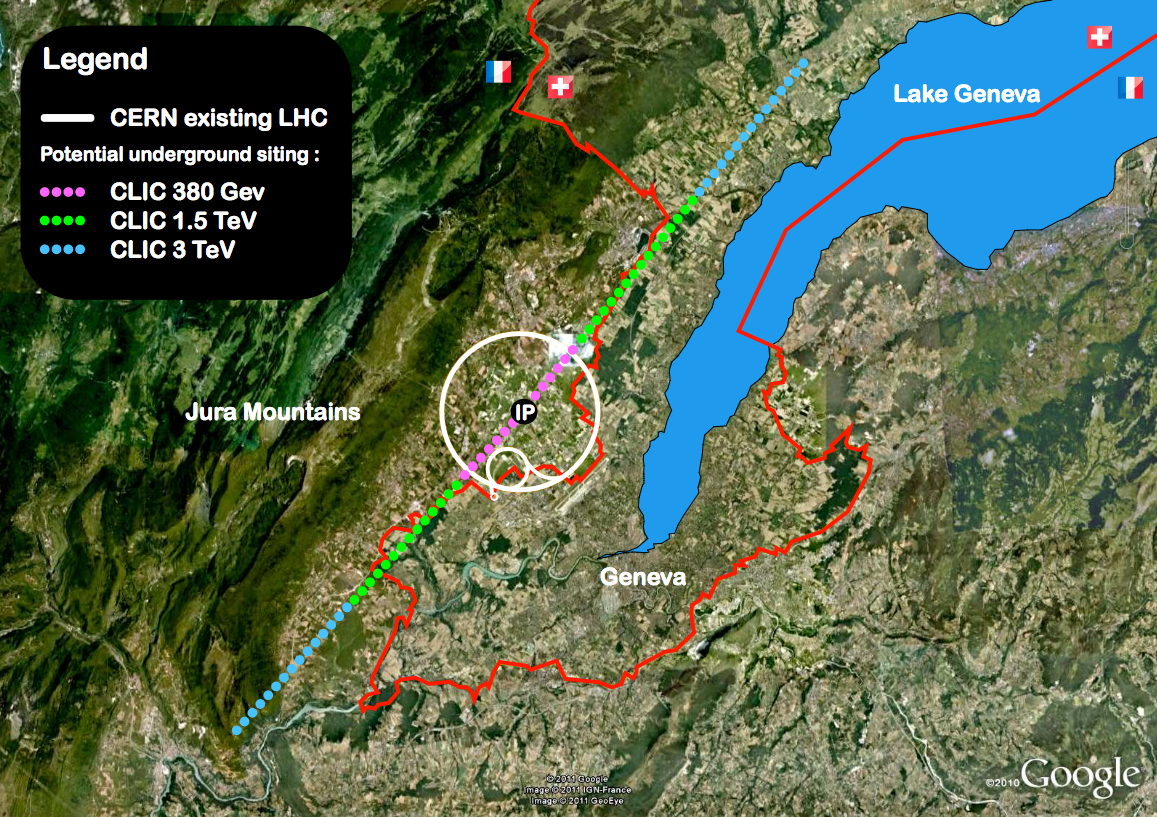
\includegraphics[scale=0.3]{pictures/CLIC_map}
\caption{Map of the CLIC facility, if implemented in the Geneva area.}
\label{CLIC_map}

\end{figure}


\subsection{Main parameters and main issues}

The realisation of a machine like CLIC implies many technological challenges in order to keep the power consumption and the dimension limited while matching the design goal parameters. These challenges have been faced by developing the novel \textit{two-beam acceleration scheme}, which uses a high-current and low-energy beam, the \textit{Drive Beam}, in order to generate the radio-frequency (RF) power to accelerate a low-current and high-energy beam used for the experiments, named \textit{Main Beam}. 

The Drive Beam is produced using a dedicated linac, and then the current is multiplied using a delay loop and two recombination rings, reaching a combination factor of $2\text{x}3\text{x}4=24$. This topology generates the beam with a final bunch frequency of 12 GHz. It is essential to reach the highest possible efficiency in the Drive Beam production, in order to shrink the power consumption to the smallest possible value. To reach this goal the acceleration in the linac is performed using the accelerating cavities in fully-loaded mode \cite{Corsini:791372}.

While the biggest challenge for the Drive Beam is to reach the necessary stable high current, for the Main Beam the hardest challenge is generating a beam with the smallest size possible, in order to increase the luminosity of the machine as much as possible.

The Main Beam is produced in a separate facility, where a DC-photogun system provides the initial polarised electron beam. The positron beam is generated by another electron beam hitting a target. Once both beams have been produced, they are sent to the next accelerating stages, which are composed of linacs to raise the beam energy and of damping rings to reduce the emittances. 

The detailed description of the Main Beam production and the Drive Beam recombination process can be found in \cite{CLIC:cdr}. The working principle has been demonstrated in the CTF3 \cite{CTF:drive_beam}. 

Both beams are sent to the common tunnel where the Two-beam modules are installed. The Two-beam module is composed of two principal sections, the PETS, \textit{Power Extraction and Transfer Structures}, and the accelerating structures for the Main Beam, as shown in Fig.~\ref{TBM}. The Drive Beam passes through the PETS and gets decelerated. As product of the deceleration a pulse of RF power is produced, which is transferred by a waveguide network and used to accelerate the Main Beam. In this way  an efficient acceleration of the Main Beam up to the desired energy for the experiments is possible.

Figure~\ref{CLIC_layout} shows the layout of the CLIC facility in the final energy stage.

\begin{figure}[h]
\centering

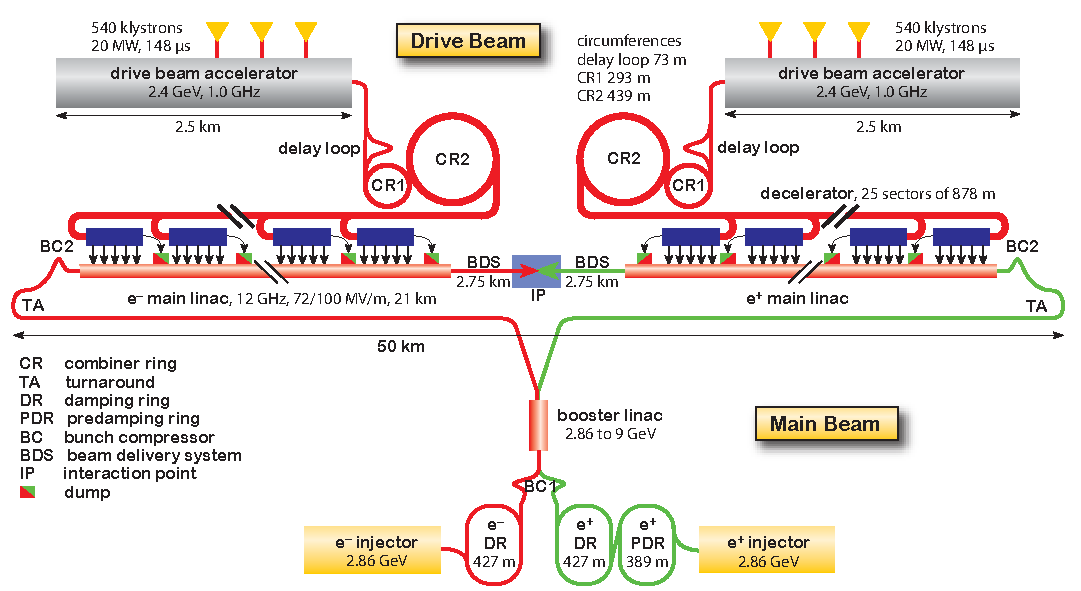
\includegraphics[scale=0.39]{pictures/CLIC_layout_3Tev}
\caption{Layout of the final stage of CLIC.}
\label{CLIC_layout}

\end{figure}

\begin{figure}

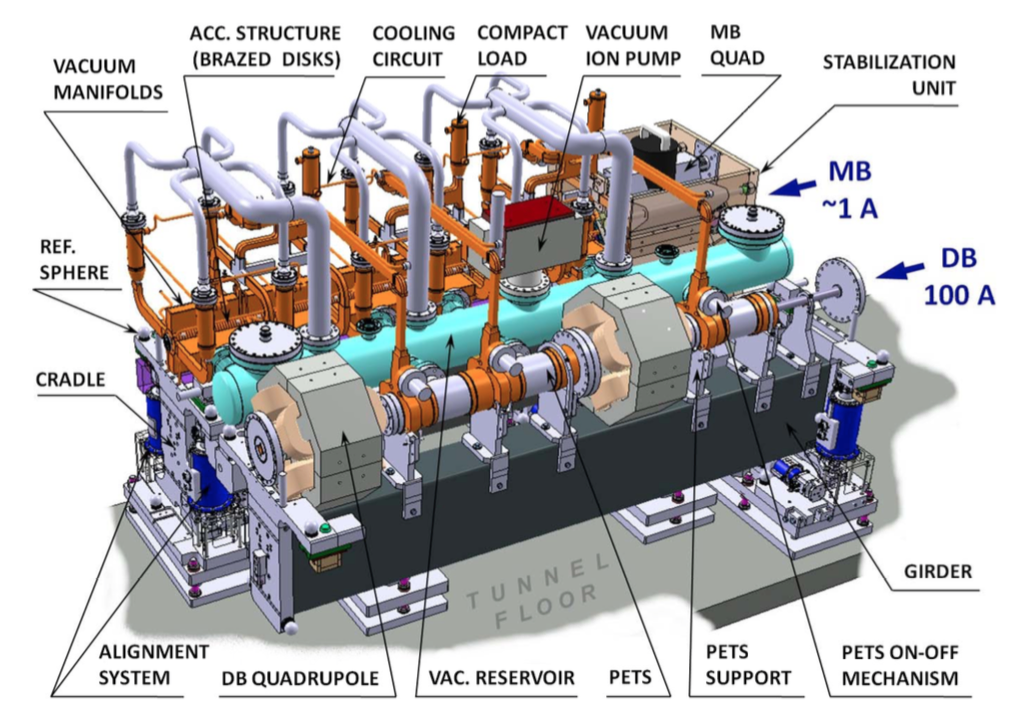
\includegraphics[scale=0.39]{pictures/TBM}
\caption{Design of a Two-beam module. }
\label{TBM}

\end{figure}







There are many issues that can affect the performance of a machine like CLIC, and need to be analysed carefully since no similar machine has been built so far. 

The main issues are:

\begin{enumerate}
\item 100 MV/m accelerating gradient: this requirement comes from the final energy of 3 TeV and the requirement of a maximum length of 50 km.
\item Breakdown rate $< 3\text{x}10^{-7}$ breakdowns per pulse per meter: this limitation comes from the limit on design luminosity loss in case of breakdown. This is the aim of this work and will be stressed in detail later.
\item Transverse wakefields limitation: wakefields have to be considered because of the short bunch spacing in the bunch train. If not limited, they are a serious issue to the luminosity.
\item Powering the accelerating structures: the klystrons on the market are not able to produce a high-power RF-pulse 150-200 ns long with a high efficiency. In order to achieve a high efficiency, it is possible to use klystrons equipped with RF pulse compression systems. This option is an alternative for the first energy stage of CLIC. For higher energies, the Drive Beam option is more cost efficient.
\item Generate the drive beam with the highest efficiency in order to contain the power consumption. Also the efficiency of the power transfer between the beams is a key issue in order to reach the energy goal.
\item Extremely small beam emittance and size: in order to match the luminosity goal with the typical low repetition rate of a linac it is necessary to squeeze the beam as much as possible, reaching the goal of 40 and 1~nm at the interaction point in the horizontal and vertical plane. This requirement includes the realisation of a nanometric alignment and vibration stabilisation system.
\end{enumerate}



The parameters in Table \ref{table_CLIC_params} have been chosen in order to match the design parameters reported in Table \ref{table_CLIC_ILC_FCC} for the top design energy.


\begin{table}[h]
  \centering
    \begin{tabular}{ l c  }
    \toprule
    \textbf{Description}						& \textbf{CLIC 3 TeV}	\\
    \midrule
    Peak luminosity [cm$^{-2}$ s$^{-1}$]			& $2.0\text{x}10^{34}$	\\
    Total site length [km]						& 48.4				\\
    Loaded accelerating gradient [MV/m]			& 100	\\
    Main LINAC RF frequency	[GHz]			& 12	\\
    Number of particles per bunch				& $3.7\text{x}10^{9}$ \\
    Bunch separation [ns]						& $0.5$ \\
    Bunches per train							& $312$ \\
    Beam pulse duration [ns]					& $156$ \\
    $\epsilon^*_x \, / \, \epsilon^*_y$ [$\mu$m]/[nm]	& $0.66/20$ \\  
    $\sigma^*_x\, / \, \sigma^*_y$ [nm]			& $40/1$	\\
    \bottomrule
    \end{tabular}
  \caption{CLIC main parameters in the final stage}
\label{table_CLIC_params}
\end{table}







\subsection[CTF3]{The CLIC Test Facility 3}

To prove that the CLIC scheme is a feasible and a reliable technology to build a functional collider, a number of tests have to be conducted since no accelerators using the Two-beam acceleration concept have been built. The CLIC Test Facility 3 has been built and operated at CERN in order to demonstrate experimentally:

\begin{itemize}
\item The feasibility of the Drive Beam generation with a frequency of 12~GHz, performing the beam recombination by means of  a delay loop and a combiner ring for a total multiplication factor of $2\times4 =8$.
\item The RF power production using the PETS and investigate possible issues of the Two-beam scheme.
\end{itemize}
In addition, a branch of the linac was used to perform high-gradient tests with the beam presence inside the accelerating cavity, which is the topic of this work. A more detailed description of such branch will follow in Chap. \ref{chap:setup}.
